\chapter{Trabalhos Relacionados}\label{chap:revisao}

\section{Considerações Iniciais}

Os trabalhos que mais se relacionam ao o aqui proposto são
aqueles que buscam transformar conjuntos de dados para
torná-los mais representativos para execução de uma
determinada tarefa. Esses trabalhos dividem-se basicamente
em dois grupos: métodos de redução de dimensionalidade e
métodos de construção interativa de atributos. 

A seguir, na Seção~\ref{sec:rd}, apresenta-se uma discussão
sobre os métodos de redução de dimensionalidade, com um
enfoque especial para métodos interativos. Na
Seção~\ref{sec:tr}, apresenta-se um levantamento sobre
pesquisas em construção interativa de atributos, um tema que
não conta com uma literatura tão vasta quanto à dos métodos
de redução, mas que tem ganhado popularidade nos últimos
anos. 

\section{Redução de Dimensionalidade}\label{sec:rd}

O problema de reduzir a dimensionalidade de conjuntos
de dados pode ser descrito da seguinte forma: dado um
conjunto de dados representado por uma matriz $\textbf{X}$
composta por $n$ vetores $\textbf{x}_i~(i \in
\{1,2,...,n\})$ $m-$dimensionais, deseja-se encontrar uma
transformação $t: \textbf{X} \rightarrow \textbf{Y}$, em que
$\textbf{Y}$ é uma matriz composta por $n$ vetores
$\textbf{y}_i~(i \in \{1,2,...n\})$ de dimensionalidade $p$
($p < m$).  Normalmente $p \ll m$ e, idealmente, $p$
equivale à  \emph{dimensionalidade intrínseca dos dados}\footnote{A
dimensionalidade intrínseca dos dados é o conjunto
mínimo de variáveis necessárias para descrever as
propriedades dos dados~\cite{Fukunaga1990}.}, fazendo
com que $t$ mantenha em $\textbf{Y}$ o máximo das
propriedades de $\textbf{X}$ quanto for possível. 

Um dos principais objetivos da redução de dimensionalidade é
amenizar os efeitos da \emph{maldição da
dimensionalidade}\footnote{A maldição da dimensionalidade foi
    um termo introduzido por \citet{Bellman1961} para se
    referir aos problemas que surgem ao lidar com conjuntos
    de dados com um elevado número de dimensões (centenas ou
    milhares). Sua maior implicação é a falta de
separabilidade entre elementos que se encontram em um espaço
de alta dimensão~\cite{Kouiroukidis2011}.} e com isso fazer
com que os métodos que operam sobre os dados tenham uma
melhor eficiência e um menor custo
computacional~\cite{Maaten2009}.  \citet{Konig2000}, por
exemplo, apresenta melhorias na precisão de sistemas de
classificação e no desempenho de sistemas de reconhecimento
automático ao preceder os procedimentos com um processo de
redução de dimensionalidade. Até mesmo outras melhorias não
tão diretas podem ser alcançadas por meio do uso de técnicas
de redução.  Trata-se do caso do mesmo trabalho apresentado
por \citet{Konig2000}, onde métodos de redução de
dimensionalidade são utilizados para reduzir a complexidade
de projetos de circuitos integrados, resultando em uma
redução na área e no consumo de energia dos circuitos. 

Uma outra utilidade dos métodos de redução de
dimensionalidade é viabilizar a construção de representações
visuais de dados multidimensionais, permitindo que sejam
mapeados em um espaço bidimensional (tela computador).
Representações visuais têm sido fundamentais para análises
exploratórias de dados, principalmente em investigações
iniciais, onde não
se conhece as propriedades dos dados~\cite{Kaski2011}. 

A literatura em redução de dimensionalidade é extensa e os
métodos desenvolvidos apresentam grande diversidade em
relação a aspectos matemáticos e computacionais. Para 
uma melhor organização, esta seção foi dividida em duas
subseções. Na Subseção~\ref{ss:auto} busca-se descrever
sucintamente os métodos automáticos e apresentar suas
limitações, evidenciando que a falta da participação
do usuário no processo faz com que muitas vezes os
resultados obtidos não sejam facilmente compreendidos. Já a
Subseção~\ref{ss:int}, apresenta os métodos que permitem ao
usuário participar no processo de redução de
dimensionalidade por meio de interações com representações
visuais. 

\subsection{Métodos Automáticos}\label{ss:auto}

A redução de dimensionalidade automática pode ser realizada
seguindo duas abordagens~\cite{Pudil1998}. A primeira
transforma os atributos de entrada em um novo conjunto de
dimensões que busca conservar propriedades ou
relacionamentos do conjunto original. Por extrair um novo
conjunto de atributos a partir dos originais, esta abordagem
recebe o nome de extração de características (\emph{feature
extraction}). Já a segunda abordagem busca selecionar quais
dos atributos do conjunto de dados são realmente relevantes
para as análises. Como os dados não são
modificados, esta segunda abordagem é chamada de seleção de
características (\emph{feature selection}). Ambas 
abordagens serão discutidas a seguir.

\subsubsection{Extração de Características}

Como apresentado por~\citet{Maaten2009}, existe uma grande
variedade de métodos de extração de características. Não é
intuito desta subseção detalhar cada uma dessas técnicas e
levantar suas limitações particulares, mas sim ilustrar a
limitação comum que a maioria apresenta, isto é, retornar
resultados pouco intuitivos para o usuário e impedi-lo de
interagir com os dados. Para este fim, o conjunto de dados
fictício apresentado na Tabela~\ref{tab:at} será utilizado como
exemplo.

\begin{table}[htbp] 
    \footnotesize
\caption{Conjunto de dados fictício. Os valores foram
estabelecidos arbitrariamente e não apresentam
necessariamente alguma relação com índices oficiais.}
    \begin{center}
    \begin{tabular}{|l|C{1.3cm}|C{1.2cm}|C{2.2cm}|C{1.8cm}|C{1.5cm}|C{2.5cm}|}
        \cline{2-7} \multicolumn{1}{c|}{\textbf{\textit{}}} &
        \textbf{\textit{padrão}} & \textbf{\textit{clima}} &
        \textbf{\textit{gastronomia}} & \textbf{\textit{segurança}}
        & \textbf{\textit{recepção}} & \textbf{\textit{infraestrutura}}
        \\ \hline 
        \textbf{Alemanha} & 8 & 3 & 2 & 8 & 3 & 9 \\ \hline
        \textbf{Brasil} & 5 & 8 & 7 & 3 & 8 & 3 \\ \hline 
        \textbf{Croácia} & 5 & 6 & 6 & 6 & 5 & 6 \\ \hline 
        \textbf{Espanha} & 7 & 9 & 9 & 5 & 8 & 8 \\ \hline 
        \textbf{França} & 8 & 4 & 7 & 7 & 1 & 8 \\ \hline
        \textbf{Itália} &  7 & 8 & 9 & 5 & 7 & 7 \\ \hline 
        \textbf{Marrocos} & 4 & 7 & 8 & 2 & 9 & 2 \\ \hline
        \textbf{México} & 2 & 5 & 5 & 2 & 7 & 3 \\ \hline
        \textbf{Nigéria} & 2 & 4 & 4 & 2 & 7 & 2 \\ \hline
        \textbf{Peru} & 5 & 6 & 6 & 3 & 6 & 4 \\ \hline
        \textbf{Rússia} & 6 & 2 & 2 & 3 & 3 & 6 \\ \hline
        \textbf{Turquia} & 5 & 8 & 9 & 3 & 9 & 3 \\ \hline
    \end{tabular} 
    \end{center} 
    \label{tab:at} 
\end{table}

Um dos primeiros métodos desenvolvidos para a redução de
dimensionalidade trata-se da análise de componentes principais
(PCA)~\cite{Pearson1901}, sendo que até hoje é um dos mais
utilizados~\cite{Joll2002}. Neste método, as dimensões
extraídas, ou componentes, são combinações lineares das
dimensões originais, onde cada uma busca capturar
características distintas das outras. 

A Tabela~\ref{tab:at-pcs} apresenta o resultado obtido pela
técnica PCA para os dados da Tabela~\ref{tab:at}. Nota-se a
dificuldade em interpretar o resultado obtido, pois
aparentemente os componentes extraídos não apresentam
nenhuma relação com os dados originais. Com base somente
nesse resultado não é possível, por exemplo, compreender
quais atributos foram combinados para a obtenção de tais
componentes.

\begin{table}[!h]
    \footnotesize
    \caption[Resultado de PCA]
    {Resultado obtido pela técnica PCA para os dados da
    Tabela~\ref{tab:at}. As novas dimensões são combinações lineares das dimensões
originais.}
    \begin{center}
        \begin{tabular}{|l|c|c|c|c|c|c|}
            \hline
            & \multicolumn{1}{l|}{\textbf{\textit{Comp.1}}}
            & \multicolumn{1}{l|}{\textbf{\textit{Comp.2}}}
            & \multicolumn{1}{l|}{\textbf{\textit{Comp.3}}}
            & \multicolumn{1}{l|}{\textbf{\textit{Comp.4}}}
            & \multicolumn{1}{l|}{\textbf{\textit{Comp.5}}}
            & \multicolumn{1}{l|}{\textbf{\textit{Comp.6}}}
            \\ \hline
    \textbf{Alemanha} & -8.3095 & 0.5446 & 1.9864 & -0.3819 & -0.8144 & 0.0869 \\ \hline
    \textbf{Brasil} & 3.4480 & -0.9062 & 0.2499 & 0.2469 & -0.6788 & -1.0215 \\ \hline
    \textbf{Croácia} & -1.7908 & -0.8416 & 0.0145 & -1.5911 & 0.1811 & -0.4065 \\ \hline
    \textbf{Espanha} & 0.4513 & -5.7962 & 1.2968 & 0.3819 & 0.9095 & 0.1914 \\ \hline
    \textbf{França} & -6.6956 & -2.0063 & -2.7319 & -0.2799 & -0.0306 & 0.1222 \\ \hline
    \textbf{Itália} & 0.0796 & -4.7684 & 0.0922 & 0.3013 & 0.3266 & 0.2819 \\ \hline
    \textbf{Marrocos} & 5.1923 & -0.0863 & -0.4045 & 0.2746 & -0.5028 & 0.3295 \\ \hline
    \textbf{México} & 2.7158 & 3.3806 & 0.0858 & -0.6728 & 1.1078 & -0.0102 \\ \hline
    \textbf{Nigéria} & 2.5911 & 4.8643 & 0.1585 & -0.6316 & 0.2394 & 0.1379 \\ \hline
    \textbf{Peru} & 0.9130 & 0.6241 & -0.4731 & 0.4676 &
            0.0180 & -0.6031 \\ \hline
    \textbf{Rússia} & -4.5417 & 4.3595 & -0.0156 & 1.7600 & 0.4539 & -0.1299 \\ \hline
    \textbf{Turquia} & 4.5991 & -2.2306 & -0.3223 & 0.1513 & -0.6417 & 0.2367 \\ \hline
        \end{tabular}
    \end{center}
    \label{tab:at-pcs}
\end{table}

Em PCA, os componentes são gerados em uma ordem decrescente
de importância, de modo que o primeiro captura mais
informação dos dados que o segundo e assim por diante.
Deste modo, a redução de dimensionalidade em si ocorre ao se
manter os $k$ primeiros componentes gerados pelo método. Em
tarefas de visualização, por exemplo, é comum escolher $k=2$
para manter somente os dois primeiros componentes e então
criar uma representação bidimensional dos elementos. Uma
possibilidade menos arbitrária para definir $k$ é analisar a
parcela da variância dos dados que cada componente captura.
Tal análise pode ser realizada com o auxílio de gráficos,
como o apresentado na Figura~\ref{fig:scree}. Com base neste
gráfico, nota-se que os dois primeiros componentes capturam
grande parte da variância (aproximadamente $92\%$). No
entanto, mesmo com o auxílio de tais recursos o usuário
acaba dependendo de medidas estatísticas para medir valores
que muitas vezes podem ser subjetivos.

\begin{figure}[h!]
    \centering
    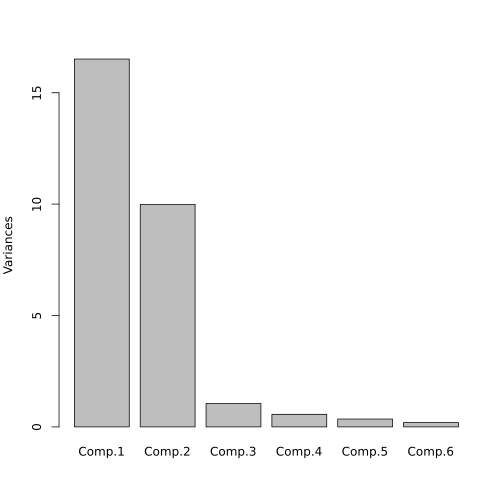
\includegraphics[width=12cm]{images/scree.pdf}
    \caption[Variância capturada pelos PCs]
        {Variância dos dados capturada por cada componente
        para os dados da Tabela~\ref{tab:at}. Os
        dois primeiros componentes capturam cerca de $92\%$
        da variância.}
    \label{fig:scree}
\end{figure}

Quando existem relações não lineares entre os atributos, PCA
não é capaz de capturá-las. Em situações como esta, métodos
não lineares como \textit{Multimensional Scaling}
(MDS)~\cite{Cox2002} e \textit{Self Organizing Maps}
(SOM)~\cite{Kohonen1990} podem ser utilizados para uma maior
eficácia. Porém, independentemente de quais técnicas se
sobressaem sobre as outras, uma limitação que os métodos de
extração compartilham entre si é a dificuldade em se
compreender o resultado obtido, ou seja, o espaço
dimensional gerado tem pouco significado para o usuário. 

Como pode ser observado na Tabela~\ref{tab:at-pcs}, não
existe uma correspondência direta entre as dimensões
extraídas e as originais. Logo, o usuário pode ter
dificuldades em associar quais características dos dados
foram responsáveis por aquele resultado. A seguir
apresenta-se uma abordagem alternativa que leva em
consideração tal problema e busca manter uma correspondência
entre o espaço dimensional reduzido e o original.

\subsubsection{Seleção de Características} 

O objetivo dos métodos de seleção de características é
encontrar o subconjunto  dos atributos de entrada mais
adequado para a aplicação em estudo. Assim, busca-se
identificar e eliminar atributos
redundantes~\cite{Kohavi1997} ou que não apresentem relação
com o fenômeno investigado~\cite{Nilsson2007}.  Por exemplo,
em tarefas de classificação supervisionada, pode-se
determinar a importância de um atributo ao se avaliar sua
correlação em respeito ao atributo classe, de modo que
atributos com altos valores de correlação são de maior
importância. Os métodos de seleção dividem-se basicamente
em \emph{filtros}, \emph{wrappers} e \emph{métodos
embutidos}~\cite{Guyon2003}. 

Filtros utilizam um atributo alvo como referência e
determinam, a partir de alguma medida de correlação, quanto
cada atributo se relaciona com esta referência. A filtragem
é realizada por meio da eliminação de atributos que apresentam relação
menor do que um valor fixado. Uma das desvantagens de
filtros é que pelo fato de considerarem somente relações
par-a-par, não são capazes de detectar dependências
indiretas entre os atributos. 

O funcionamento de \emph{wrappers} e métodos embutidos
consiste em realizar uma busca sobre subconjuntos candidatos
e tomar como resultado o subconjunto que resulta na melhor
precisão de um algoritmo de predição. O caso completo
trata-se da avaliação de $2^m$ subconjuntos, onde $m$
corresponde ao número de atributos do conjunto de entrada.
Tal situação equivale a um problema
$np$-completo~\cite{Amaldi1998}, consequentemente para
grandes conjuntos de dados a solução ótima não pode ser
obtida em tempo viável, exigindo assim a adoção de alguma
heurística. São justamente essas heurísticas que definem os
diferentes métodos que podem ser utilizados. De um modo
geral, a distinção entre \emph{wrappers} e métodos embutidos
vem de que os primeiros enxergam o método de predição como
uma ``caixa-preta'', se interessando somente pelo resultado
obtido e permitindo que diferentes preditores sejam
aplicados sem a necessidade de modificar o método de
seleção. Já os métodos embutidos são incorporados às etapas
de treinamento dos preditores, sendo assim específicos para
cada situação. 

Em comparação aos métodos de extração de características,
os métodos de seleção apresentam a vantagem de que o
resultado obtido é mais intuitivo ao usuário, pois se trata
de um subconjunto dos atributos de entrada. Assim, se o
usuário tem certo conhecimento sobre o conjunto de entrada,
então será capaz de compreender os resultados obtidos. No
entanto, eles compartilham da mesma natureza caixa-preta dos
métodos de extração. Isto é, impedem qualquer tipo de 
interação durante o processo de redução, impedindo que o
usuário contribua com seu conhecimento sobre o domínio e
compreenda quais características dos seus dados foram
responsáveis por aquele resultado. A seguir apresenta-se um
levantamento dos trabalhos que inserem o usuário no
processo de redução para contornar essa limitação.

\subsection{Métodos Interativos}\label{ss:int}

Métodos visuais que permitem a interação do usuário ganharam
popularidade nos últimos anos~\cite{State2012}.
Grande parte deste sucesso deve-se ao uso efetivo
da capacidade preemptiva da visão humana. Foi demonstrado
que quando os dados são representados por alguma forma
gráfica, o ser humano é capaz de detectar e reconhecer
padrões facilmente e com rapidez~\cite{Healey1995}, mesmo em
grandes conjuntos de dados~\cite{Fodor2002}. Mas utilizar a
capacidade preemptiva da visão humana não é a única vantagem
dos métodos visuais. Permitir que o usuário participe
ativamente nos processos e na geração dos resultados é um
dos grandes benefícios desses métodos. 

A seguir serão apresentados os trabalhos desta vertente que
buscam executar redução de dimensionalidade de forma
interativa. São trabalhos que não somente fazem uso da
capacidade perceptiva humana, mas que também permitem que o
usuário participe ativamente na geração dos resultados com o
seu conhecimento sobre o domínio.

\subsubsection{Matrizes de Correlação}\label{sss:cormat}

Uma das maneiras mais utilizadas para inspecionar
relações entre dimensões são as matrizes de
correlação~\cite{Friendly2002}. A Figura~\ref{fig:bs1}
apresenta um exemplo deste tipo de representação para um
conjunto de dados de \emph{baseball}~\cite{Friendly2002}. Com base em uma
investigação visual sobre essa figura é possível levantar
algumas hipóteses sobre os dados. Observa-se, por exemplo,
uma relação direta entre os anos de carreira do jogador
(\emph{Years}) e o seu salário (\emph{logSal}), ao mesmo tempo a
experiência tem uma relação inversa com o número de erros.

\begin{figure}[h!]
    \centering
    \includegraphics[width=10cm]{images/bs1.pdf}
    \caption[Matrizes de Correlação]
    {Exemplo de matriz de correlação. A cor azul indica
    correlação positiva entre as variáveis, enquanto a
vermelha correlação negativa. A intensidade da cor é
proporcional à magnitude da correlação.}
    \label{fig:bs1}
\end{figure}

Esse tipo de representação é útil para ter uma visão
geral das relações entre pares de dimensões. No entanto,
para análises mais detalhadas, ou que exijam uma comparação
entre mais do que simplesmente pares de elementos, não é uma
representação adequada.

Devido à sua simplicidade, matrizes de correlação têm sido
adotadas por diversos métodos visuais que viabilizam a
investigação de atributos de conjuntos de dados. A
ferramenta desenvolvida por \citet{Guo2003}, por exemplo,
utiliza matrizes de correlação para apresentar as relações
entre os atributos e utiliza um método de agrupamento para
ordenar as colunas da matriz de modo a destacar grupos de
dimensões similares.

\begin{figure}[h!]
    \centering
    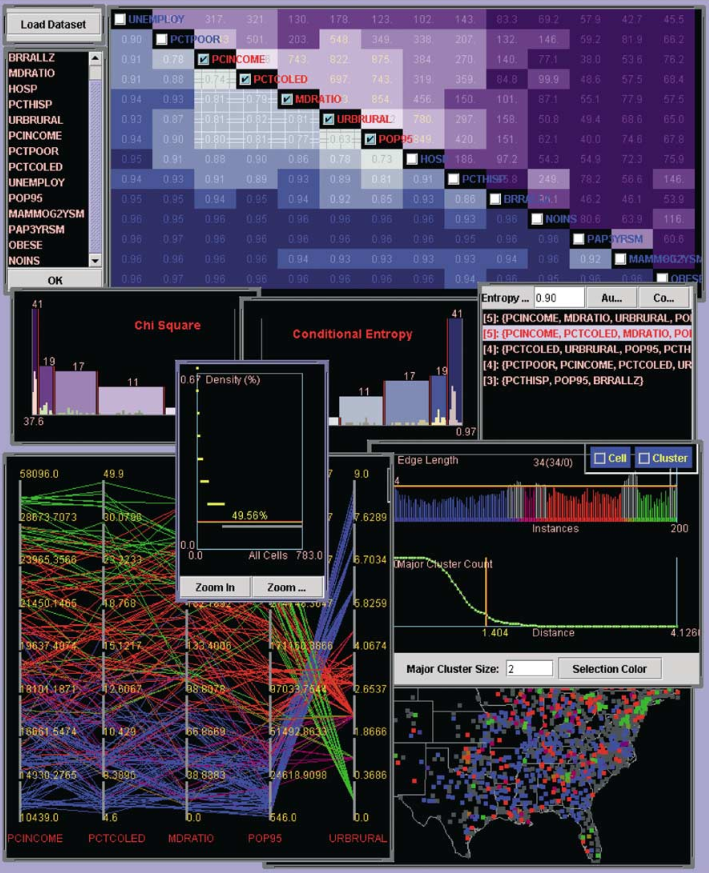
\includegraphics[width=12cm]{images/coord.png}
    \caption[Ferramenta proposta por \cite{Guo2003}]
    {Visão geral da ferramenta desenvolvida por
    \citet{Guo2003}. Imagem extraída de \cite{Guo2003}).} 
    \label{fig:coord}
\end{figure}

A Figura~\ref{fig:coord} apresenta uma visão geral da
ferramenta proposta por \citet{Guo2003}. Na parte superior
da figura encontra-se a matriz de correlação, onde o usuário
seleciona subconjuntos de atributos de interesse por meio da
seleção dos elementos correspondentes na diagonal da matriz.
Nota-se que, devido ao método de ordenação das colunas,
os grupos de dimensões similares podem ser identificados
mais facilmente. As outras visualizações são coordenadas com
as seleções do usuário e então análises mais detalhadas podem
ser realizadas para uma melhor compreensão das estruturas
presentes naquele subconjunto de atributos. 

O objetivo das matrizes de correlação não é propriamente
reduzir a dimensionalidade do conjunto de dados, mas sim
ajudar o usuário a encontrar subconjuntos de atributos com
características de interesse. Outros trabalhos
\cite{Friendly2002,MacEachren2003,RBF2004,May2011ss,Johansson2009,Ingram2010,May2011}
também adotam matrizes de correlação para atingir esse mesmo
objetivo. Eles diferem na maneira como é construída a
matriz de correlação e de quais recursos são
disponibilizados para o usuário interagir sobre os
subconjuntos de dimensões. Um problema geral desses
trabalhos é que certas análises podem exigir demasiado
esforço do usuário devido à necessidade de se explorar
individualmente cada dimensão ou avaliar par-a-par as
relações entre atributos. Com a ocorrência de dependências
não lineares este problema torna-se ainda maior e o usuário
pode se perder em suas análises e não extrair novos
conhecimentos dos resultados. 

A seguir apresenta-se alternativas às matrizes de correlação
para se apresentar medidas de correlação. Essas abordagens
fornecem mecanismos mais diretos para se reduzir a
dimensionalidade dos conjuntos de dados. 

\subsubsection{Hierarquias de Dimensões}

Em busca de construir espaços de baixa dimensionalidade mais
intuitivamente do que pelo uso de métodos automáticos,
\citet{Yang2003} desenvolveram o método de redução de
dimensionalidade chamado VHDR (\emph{Visual Hierarchical
Dimensions Reduction}). O funcionamento deste método é
ilustrado pela Figura~\ref{fig:vhdr1}. Inicialmente (1),
constrói-se uma organização hierárquica dos atributos com
base na similaridade entre as dimensões. Em seguida (2), o
usuário define os níveis da hierarquia que devem ser
considerados pela última etapa do processo. Finalmente (3), o
usuário, por meio de um método automático ou de seu
conhecimento sobre os dados, escolhe dimensões
representativas para os níveis definidos, reduzindo assim a
dimensionalidade dos dados. 

\begin{figure}[h!]
  \centering
  \begin{subfigure}[b]{0.35\textwidth}
    \centering
    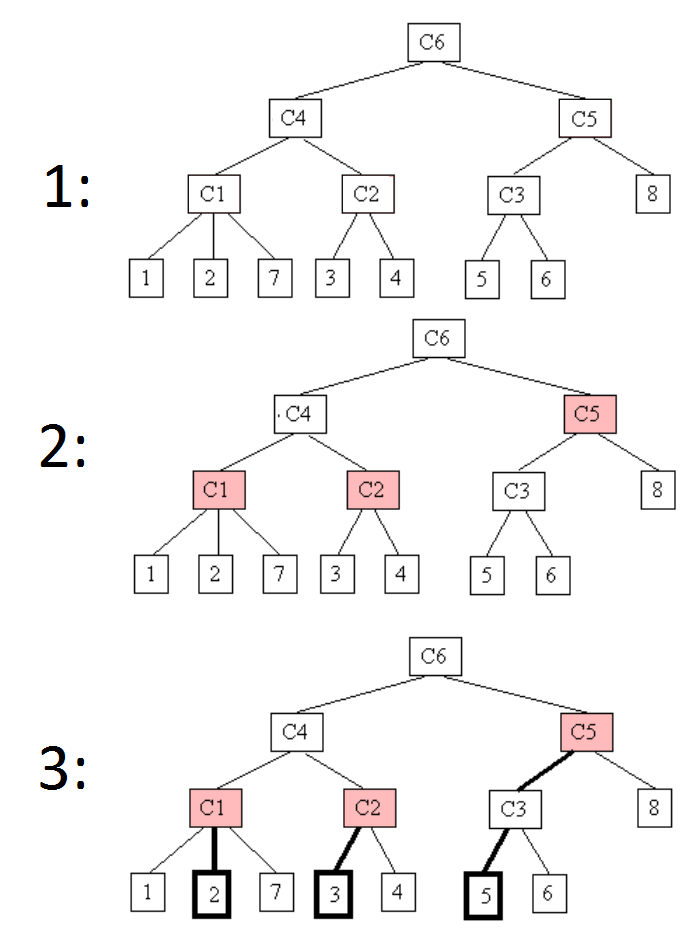
\includegraphics[width=\textwidth]{images/vhdr1.png}
    \caption{}
    \label{fig:vhdr1}
  \end{subfigure}%
  \hspace{1cm} %add desired spacing between images, e. g. ~, \quad, \qquad etc.
  \begin{subfigure}[b]{0.5\textwidth}
    \centering
    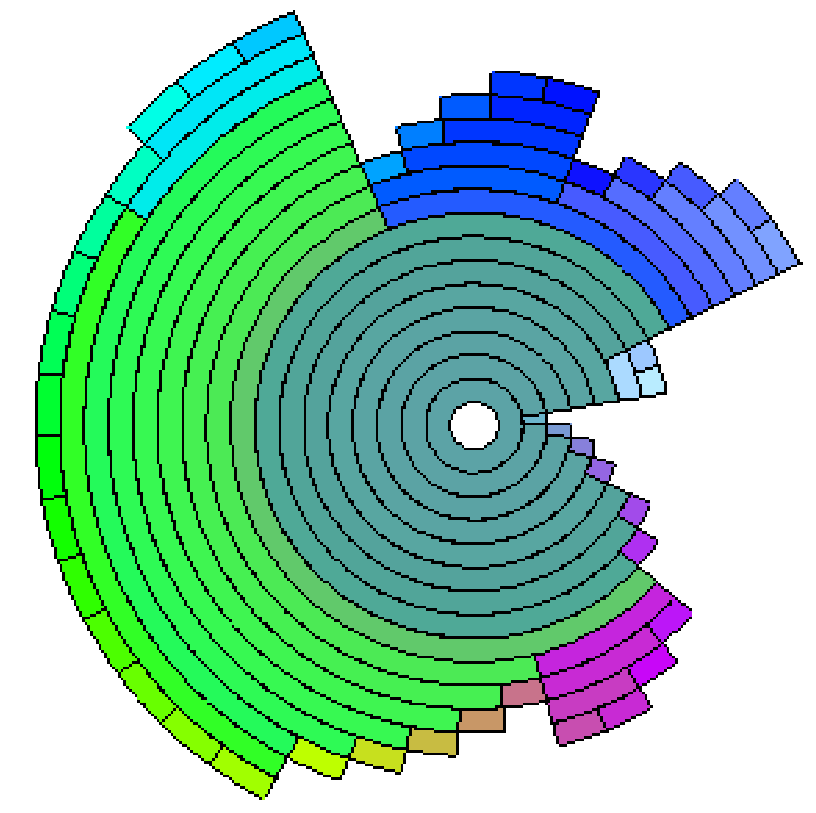
\includegraphics[width=\textwidth]{images/vhdr2.png}
    \caption{}
    \label{fig:vhdr2}
  \end{subfigure} \caption[VHDR: Visual Hierarchical
  Dimension Reduction]{Em (a) ilustra-se o funcionamento do
  VHDR. Em (b) exemplifica-se a representação gráfica adotada pelos
  autores do VHDR. Ambas imagens extraídas de
  \cite{Yang2003}.}
\end{figure}

O processo de construção da hierarquia é muito semelhante
aos algoritmos de agrupamento hierárquico. A distinção é que
agrupa-se atributos semelhantes, ao invés de itens. Deste
modo, qualquer método de agrupamento pode ser aplicado,
exigindo-se apenas que o agrupamento resulte em uma
estrutura hierárquica, no caso uma árvore, onde cada
dimensão seja representada por um nó folha da árvore. 

A representação gráfica utilizada no VHDR é a
\emph{InterRing}~\cite{Yang2002} e pode
ser observada na Figura~\ref{fig:vhdr2}. O nó raiz da árvore
é representado pelo círculo mais interno e os nós folhas
pelos elementos posicionados na borda. As cores são
utilizadas para destacar grupos de dimensões com
características em comum. 

Os autores do VHDR desenvolveram uma extensão chamada DOSFA
(\emph{Dimension Ordering Spacing and Filtering
Approach})~\cite{DOSFA} que apresenta outras abordagens para
investigar os atributos de um conjunto de dados. Mais
especificamente, eles propõem ferramentas para ordenação,
espaçamento e filtragem de atributos. As duas primeiras,
ordenação e espaçamento, não estão diretamente relacionadas
com redução de dimensionalidade. Já a filtragem de atributos
é análoga aos métodos de seleção de características. Este
mecanismo consiste em remover dimensões pouco
representativas ou redundantes, de modo que se certas
dimensões apresentam alta similaridade entre si, então
apenas uma delas é mantida, ou se certas dimensões
apresentam pouca relevância, então são descartadas. A grande
complexidade do processo de filtragem está no modo como se
define a redundância e a importância entre as dimensões. Um
método semelhante para filtragem de atributos irrelevantes
foi proposto por \citet{Artero2006}.

Tanto o VHDR quanto o DOSFA tratam todo o conjunto de dados
de maneira uniforme. No entanto, podem existir subconjuntos
nos dados com diferentes características que devem ser
analisados separadamente~\cite{May2011}. Uma maneira de
contornar este problema seria apresentar os itens
simultaneamente com a representação das dimensões, assim o
usuário poderia detectar grupos não somente nas dimensões
mas também nos itens. Os trabalhos discutidos a seguir
utilizam tal representação para reduzir a dimensionalidade
dos conjuntos de dados. Esses trabalhos servem como
inspiração para a construção das visualizações que
utilizaremos na proposta deste projeto.  

\subsubsection{Mapeamento de Elementos no Plano}

Abordando justamente o problema de se apresentar itens
simultaneamente com as dimensões de um conjunto de dados,
\citet{Yang2004} desenvolveram a ferramenta VaR (\emph{Value and
Relation}). A abordagem une os conceitos de MDS e glifos para
representar as dependências entre as dimensões de uma base
de dados. 

\begin{figure}[h!]
  \centering
  \begin{subfigure}[b]{0.5\textwidth}
    \centering
    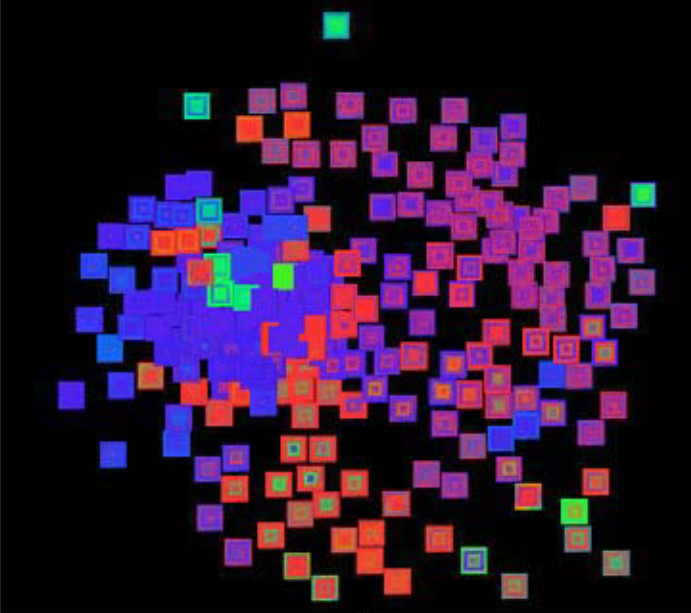
\includegraphics[width=\textwidth]{images/var1.png}
    \caption{}
    \label{fig:var1}
  \end{subfigure}%
  ~ %add desired spacing between images, e. g. ~, \quad, \qquad etc.
  \begin{subfigure}[b]{0.475\textwidth}
    \centering
    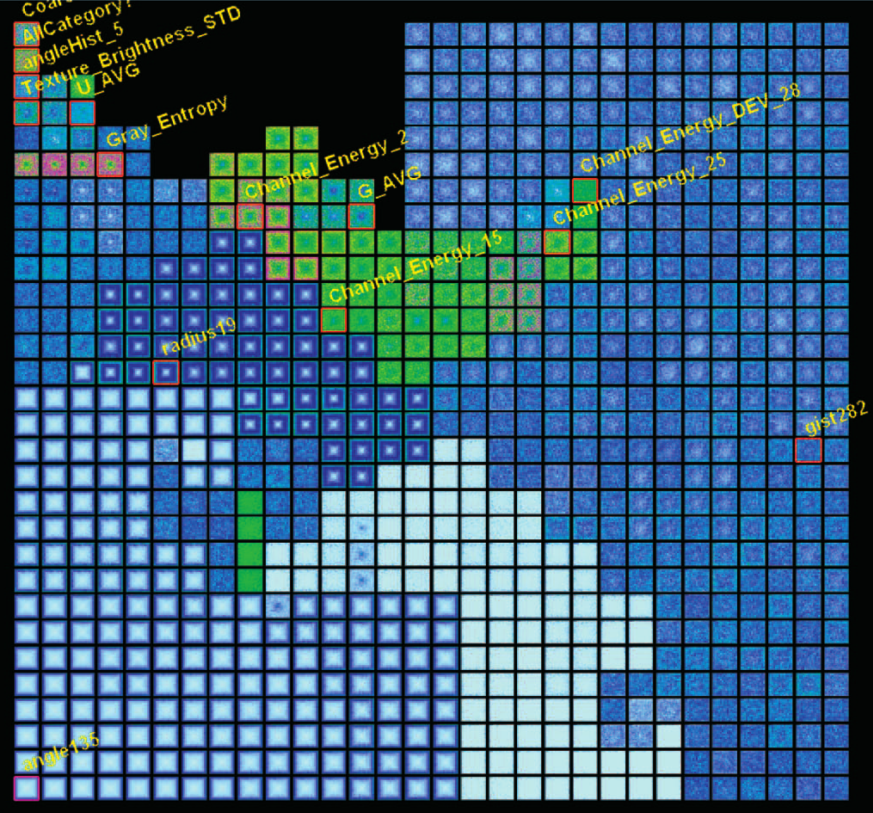
\includegraphics[width=\textwidth]{images/var2.png}
    \caption{}
    \label{fig:var2}
  \end{subfigure}
  \caption[VaR: Value and Relation]
      {Em (a) exemplifica-se a ferramenta VaR. Em (b)
          apresenta-se um exemplo da representação
          alternativa proposta como extensão da ferramenta
          VaR. Imagens extraídas de \cite{Yang2004} e
      \cite{Yang2007}, respectivamente.}
\end{figure}

Na representação visual da ferramenta VaR, cada dimensão é
representada por um glifo e seus posicionamentos refletem a
similaridade entre as dimensões, de modo que glifos que se
encontram próximos indicam atributos que apresentam alguma
relação entre si. Como mostra a Figura~\ref{fig:var1}, de
acordo com o posicionamento dos glifos no plano o usuário
pode compreender como as dimensões se relacionam entre si. O
usuário é capaz de construir espaços dimensionais reduzidos
que conservam certas características dos dados por meio de
seleções manuais sobre os dados ou pelo uso de um método automático.
Este método automático parte de uma dimensão de referência e
de um limiar definido pelo usuário e retorna as dimensões
mais semelhantes à esta referência.

O procedimento para o mapeamento das dimensões tem início
com a construção de uma matriz de distâncias que é
responsável por capturar os relacionamentos entre pares de
dimensões do conjunto de dados. Sobre esta matriz de
distâncias aplica-se uma técnica de MDS para mapear cada
dimensão em uma posição do espaço bidimensional.
Finalmente, cria-se um glifo orientado a pixels para cada
dimensão que é utilizado para representar as dimensões
no plano.

Observando a Figura~\ref{fig:var1} nota-se que o
uso de glifos faz com que ocorram sobreposições, pois cada
glifo requer um espaço relativamente grande para que seja
analisado adequadamente.  As sobreposições dificultam as
análises de regiões de interesse e podem fazer com que o
usuário alcance conclusões inválidas, devido a oclusão de
algum elemento importante.  

Para tratar o problema de sobreposição de elementos,
\citet{Yang2007} desenvolveram a extensão ilustrada na
Figura~\ref{fig:var2}, onde apresentaram alternativas para o
mapeamento dos glifos no plano. Porém, a abordagem 
proposta estabelece uma distância fixa entre os elementos e
consequentemente perde-se a informação de quanto duas
dimensões são similares entre si. Assim, o resultado obtido
pela versão original transmite melhor os relacionamentos entre
as dimensões do que a abordagem proposta na extensão. 

Apesar de a ferramenta VaR apresentar informações sobre itens
e dimensões simultaneamente, não é permitido ao usuário
interagir com os itens. Consequentemente, esta abordagem
sofre das mesmas limitações das ferramentas apresentadas
anteriormente, ou seja, não é capaz de lidar com  
características locais em subconjuntos dos dados. Um outro
aspecto importante que os próprios autores mencionam em
relação ao uso de glifos é que os usuários têm dificuldade
em comparar glifos que se encontram afastados. 

\begin{figure}[h!] \centering
    \begin{subfigure}[b]{0.45\textwidth}
    \centering
    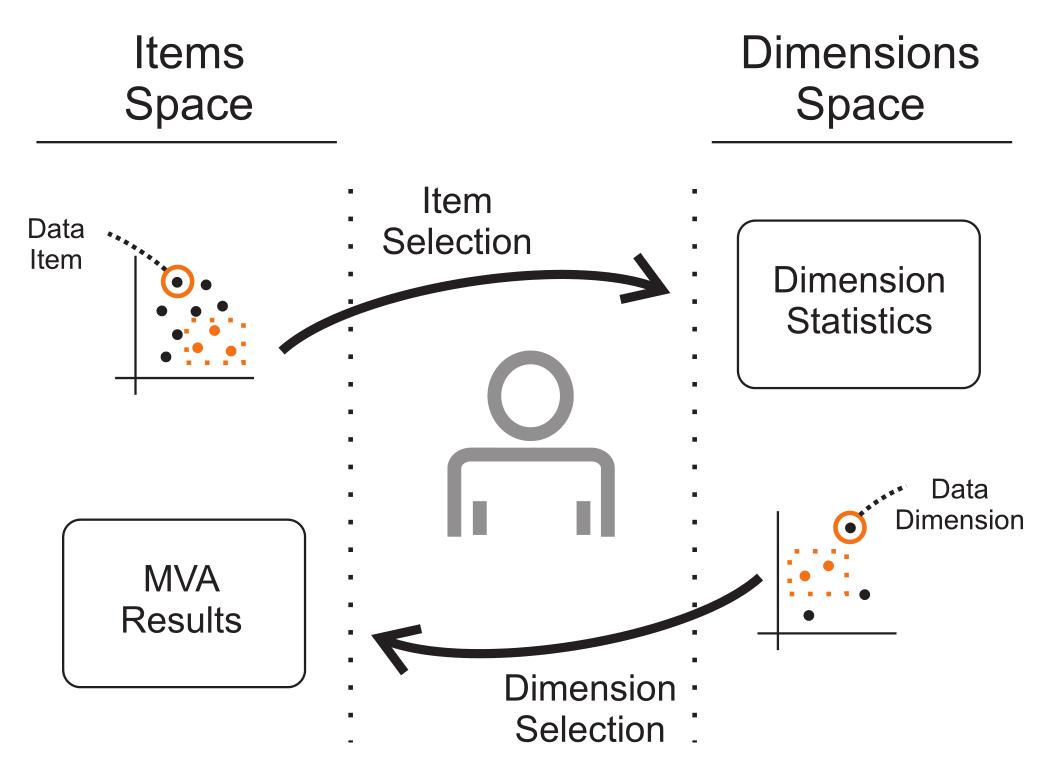
\includegraphics[width=\textwidth]{images/bd1.png}
    \caption{}
    \label{fig:bd1}
  \end{subfigure}%
  \begin{subfigure}[b]{0.55\textwidth}
    \centering
    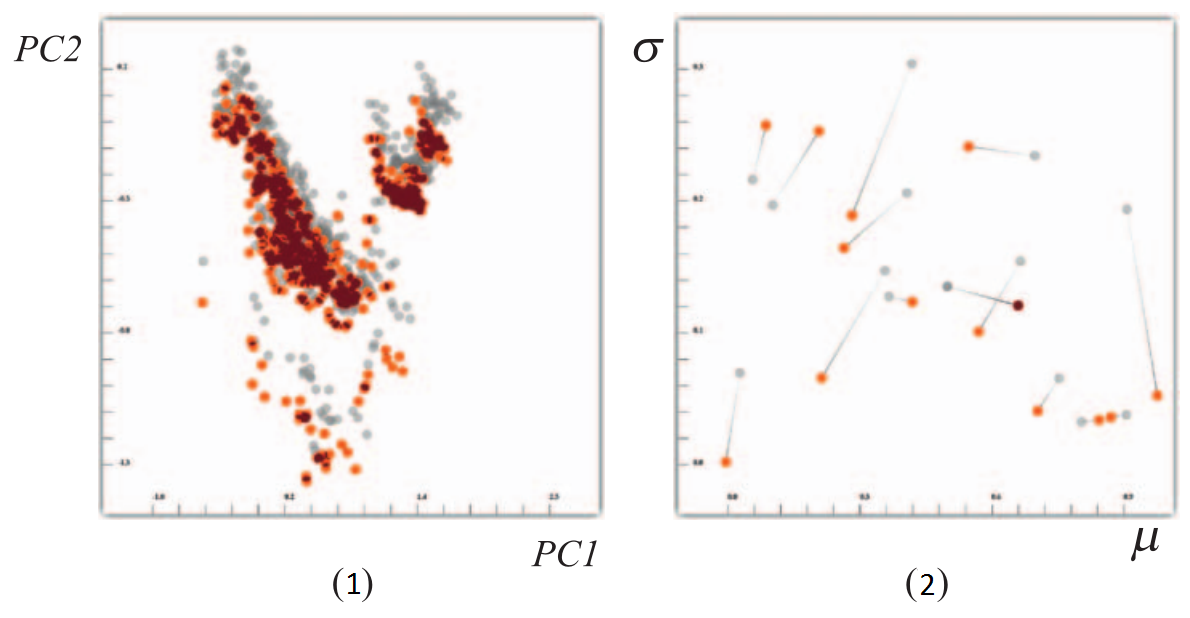
\includegraphics[width=\textwidth]{images/bd2.png}
    \caption{}
    \label{fig:bd2}
  \end{subfigure}
  \caption[Brushing Dimensions]
  {Em (a) ilustra-se o conceito principal do trabalho de
  \citet{Turkay2011}, \emph{Brushing Dimensions}. Em (b) à
  esquerda (1) apresenta-se a representação visual dos itens
  e na direita (2) a das dimensões. Imagens extraídas de
  \cite{Turkay2011}}
  \label{fig:bd}
\end{figure}

O trabalho proposto por \citet{Turkay2011}, \emph{Brushing
Dimensions} (BD), cobre essa limitação da ferramenta
VaR, pois permite aos usuários interagir tanto com as
dimensões dos conjunto de dados quanto com os itens.  Como
pode ser observado na Figura~\ref{fig:bd} o usuário pode
realizar seleções em ambas direções. Semelhantemente à
ferramenta VaR, as representações visuais do BD são baseadas
em mapeamentos de elementos no plano. As representações dos
itens são construídas com base em métodos automáticos, como
PCA, e as das dimensões por medidas estatísticas, como média
e variância. Este modo de posicionamento das dimensões é uma
das limitações da ferramenta, pois ao desconsiderar medidas
par-a-par, como correlação, a visualização não apresentará
dependências entre os atributos. O principal mecanismo de
interação da ferramenta BD é a seleção que se reflete em
outras visões e permite que se visualize, por exemplo,
variações na importância de um atributo em diferentes
subconjuntos dos dados. Uma das limitações de ambos os
métodos, VaR e BD, é não permitir que o usuário construa
novas dimensões com base nas originais ou com base em seu
conhecimento.

Uma questão inerente de se mapear elementos de um espaço de
alta dimensionalidade em um plano, sejam os elementos itens
ou dimensões, é que não há garantias de que o mapeamento
seja válido. Em casos onde a dimensionalidade intrínseca dos
dados for maior do que a do espaço alvo, então poderá haver
sobreposição de elementos sem necessariamente significar que
os elementos sobrepostos sejam realmente semelhantes. Ambos
VaR e BD não atentam para esta questão, mas
\citet{Ingram2010} desenvolveram a ferramenta
\emph{DimStiller} buscando construir mapeamentos de
dados multidimensionais levando em consideração este
problema. 

\begin{figure}[h!]
    \centering
    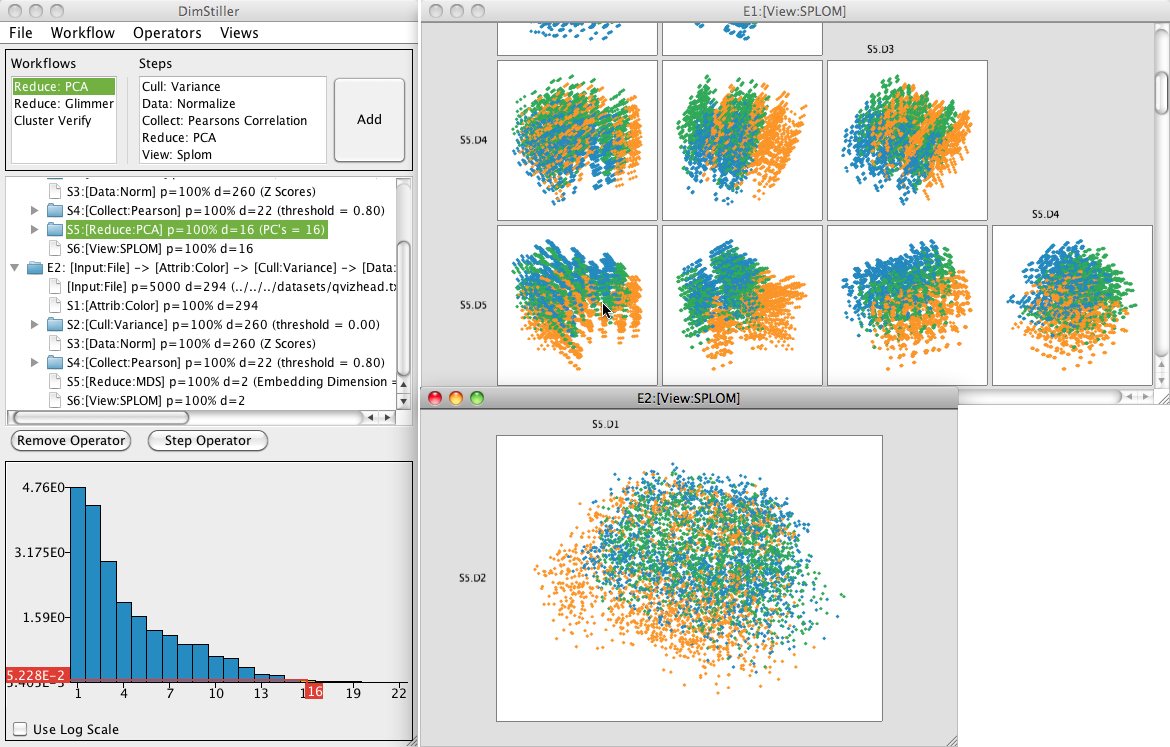
\includegraphics[width=16cm]{images/ds.png}
    \caption[DimStiller]
    {Abordagem proposta pela ferramenta \emph{DimStiller}
    para criar mapeamentos de dados multidimensionais
interativamente. Imagem extraída de \cite{Ingram2010}}
    \label{fig:ds}
\end{figure}

A Figura~\ref{fig:ds} ilustra a ferramenta
\emph{DimStiller}. Pelo gráfico de barras (janela canto
inferior esquerdo) o usuário reconhece a dimensionalidade
intrínseca dos dados e para os limites da redução de
dimensionalidade. O mapeamento resultante da redução é
apresentado em um gráfico dos dois componentes principais
(janela canto inferior direito). De acordo com esta
visualização, não existem estruturas de interesse nos dados.
No entanto, ao observar mapeamentos com outros componentes
da redução (janela canto superior direito), o usuário pode
identificar padrões nos dados.

Outro aspecto importante da redução de dimensionalidade,
que muitas vezes não é levado em consideração, é que
dependendo do método adotado, diferentes características dos
dados podem ser mantidas e outras perdidas. Este problema é
abordado no trabalho de \citet{Johansson2009}, onde por meio
de gráficos de perda de informação para diferentes medidas,
o usuário pode entender quais características dos seus dados
são mantidas e perdidas ao longo do processo de redução. 

O trabalho de \citet{Johansson2009} e \cite{Ingram2010} 
fornecem meios para o usuário avaliar a incerteza dos
resultados. Apresentam aos
usuários os fatores que podem resultar em interpretações
ambíguas dos resultados e na perda de possíveis informações
de interesse. Tal característica não é presente em muitas das
ferramentas de visualização atuais, mas tem se tornado cada
vez mais uma exigência~\cite{Dill2012}.

As ferramentas de redução de dimensionalidade não são
restritas a totalmente automáticas ou integralmente
interativas. Abordagens mistas podem ser adotadas, como é o
caso dos trabalhos discutidos a seguir.

\subsubsection{Visualização de Métodos Automáticos}

Existem métodos que não fazem uso de representações
visuais para realizar a redução de dimensionalidade em si,
mas sim para tornar os métodos automáticos mais
compreensivos. Eles buscam incluir a participação do usuário
nesse processo para tornar esses métodos ``caixas-pretas'' mais
intuitivos. 

\begin{figure}[h!]
    \centering
    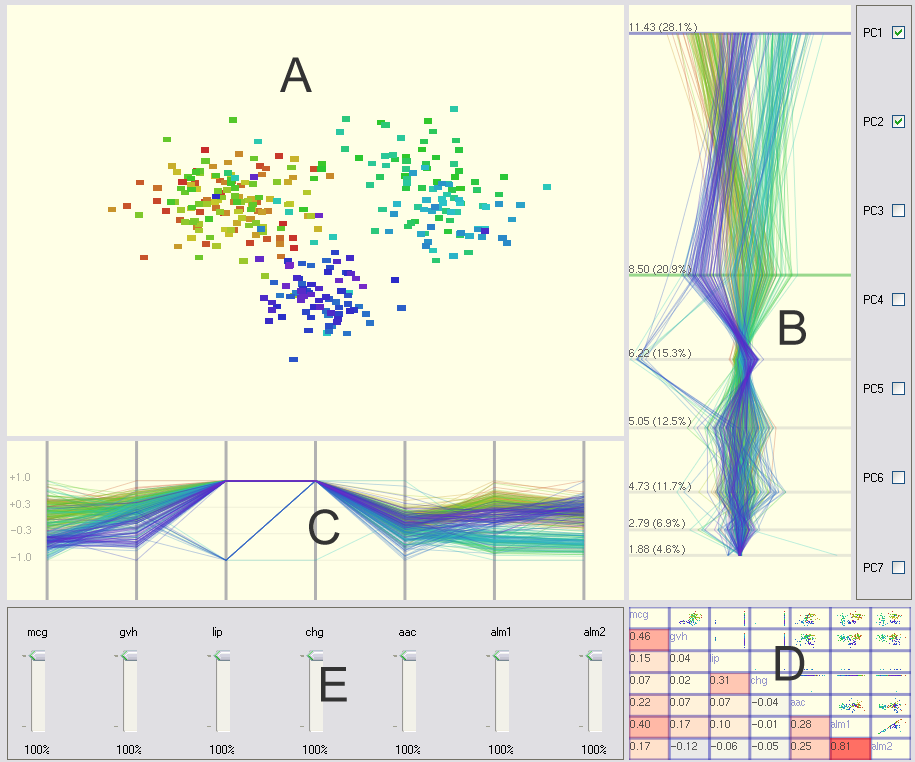
\includegraphics[width=12cm]{images/ipca.png}
    \caption[iPCA]{Ilustração da ferramenta iPCA. Imagem
    extraída de ~\cite{Jeong2009}}
    \label{fig:ipca}
\end{figure}

No contexto de extração de características, a ferramenta
iPCA~\cite{Jeong2009} provê meios para o usuário manipular a
importância de cada atributo na técnica PCA e, assim, ser
capaz de entender mais facilmente as transformações
realizadas sobre os dados. O funcionamento dessa ferramenta
é ilustrado na Figura~\ref{fig:ipca}. Em (A) apresenta-se o
mapeamento dos elementos no plano utilizando dois
componentes principais selecionados pelo usuário. (B) e (C)
referem-se a visualizações dos dados originais e
transformados, respectivamente. Em (D) é apresentada uma
matriz de correlação. O principal mecanismo de interação é
indicado por (E), o qual permite ao usuário definir a
contribuição de cada atributo no resultado final.

Similarmente, \citet{Williams2004}
permitem que o usuário guie o processo de redução de
dimensionalidade a partir de métodos MDS ao escolher regiões
de interesse para se concentrar os esforços computacionais.
Neste mesmo sentido, \citet{Schreck2008} desenvolveram uma
ferramenta que permite ao usuário monitorar visualmente os
recursos computacionais utilizados pelo método SOM e definir
interativamente os parâmetros para sua execução.

As visualizações também podem ser utilizadas para tornar
métodos de seleção de características mais intuitivos. O
trabalho de \citet{Dy2000}, por exemplo, possibilita que o
usuário adicione ou remova atributos interativamente ao
longo do processo de redução. Por outro lado, o trabalho de
\citet{Brandoli2010} auxilia o usuário a definir os
parâmetros dos métodos de seleção de características.

Encontra-se na literatura alguns trabalhos que buscam tornar o
processo de redução de dimensionalidade mais intuitivo no
contexto de classificação de dados~\citet{Zhang2006,
Choo2010, Paiva2012}. Nesses trabalhos, a redução
de dimensionalidade reflete diretamente na qualidade das
classificações. 

Um problema das ferramentas que criam visualizações de
métodos automáticos é a necessidade do usuário ter um certo
conhecimento sobre o método utilizado para a construção da
visualização. Por exemplo, o usuário pode não fazer um uso
efetivo da ferramenta \emph{iPCA} se não compreender o significado
de  um componente principal.  Para pesquisadores da área
pode ser até pressuposto que o usuário tenha este tipo de
conhecimento, no entanto, se o objetivo for criar uma
ferramenta para o público em geral, então tal suposição 
restringe seu uso.

\section{Construção Interativa de Atributos}\label{sec:tr}

Os métodos de redução de dimensionalidade realizam
transformações sobre os dados, porém, mesmo as ferramentas
interativas de redução não permitem que o usuário modifique
os atributos livremente. A construção interativa de
atributos significa mais do que permitir que o usuário guie
as transformações sobre os dados, trata-se de permitir que o
usuário agregue seu conhecimento sobre os dados
incisivamente.

Esse tipo de abordagem ainda não conta com uma literatura
tão vasta quanto a dos métodos de redução de
dimensionalidade. Sendo que a contribuição mais relevante é a
ferramenta proposta por \citet{Gladys2013} que possibilita ao
usuário modificar os atributos de um conjunto de dados com
base na manipulação sobre amostras dos itens. Os autores
fazem uso de mapeamento de elementos no plano para permitir
interações intuitivas sobre os dados. 

A Figura~\ref{fig:ud} apresenta  o funcionamento dessa
ferramenta. Inicialmente, o usuário manipula uma amostra dos
dados buscando  agrupar elementos que considera similares.
Em seguida, as manipulações realizadas sobre a amostra são
refletidas para o conjunto de dados original, fazendo com
que este reflita a opinião do usuário em relação ao critério
de similaridade entre os elementos. Este processo pode ser
repetido até que se atinja o resultado esperado.  Observa-se
que para este exemplo a transformação do espaço foi bem
sucedida, pois foram reveladas estruturas que não
eram identificáveis no mapeamento original.

\begin{figure}[h!]
    \centering
    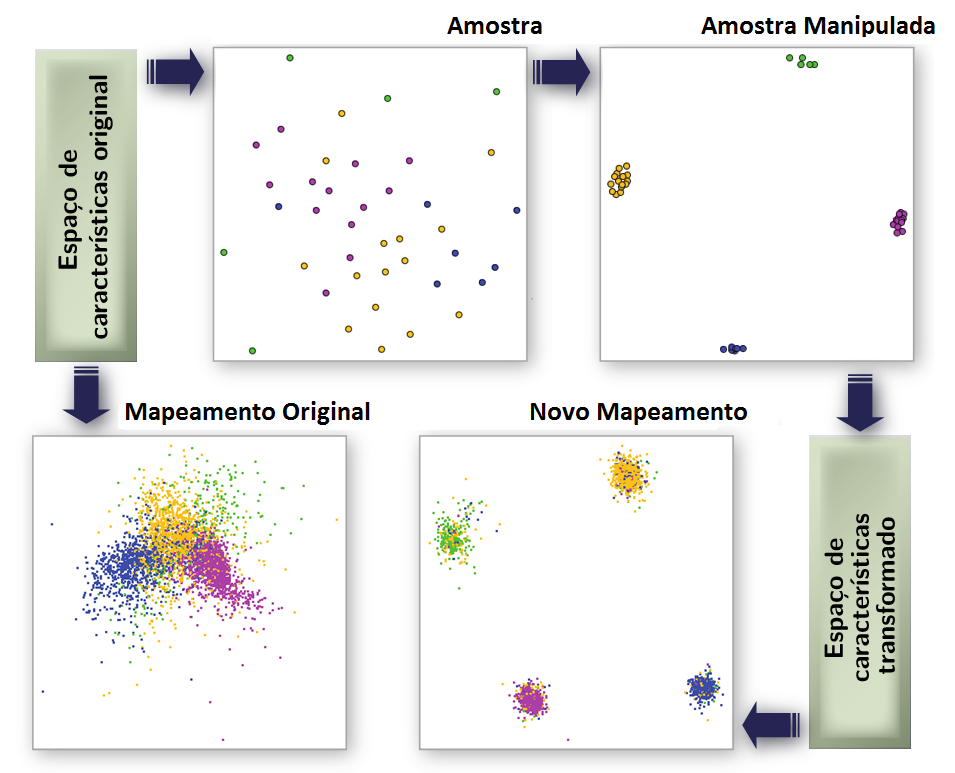
\includegraphics[width=16cm]{images/ud.png}
    \caption{Ferramenta desenvolvida por \citet{Gladys2013}.}
    \label{fig:ud}
\end{figure}

A ferramenta de \citet{Gladys2013} não constrói propriamente 
novas dimensões, mas sim modifica as
existentes para agregar o conhecimento do usuário. Ao se
transformar os dados originais o usuário pode ter
dificuldade em interpretar o resultado obtido,
semelhantemente ao que acontece com os métodos automáticos
de extração de características. Na abordagem aqui proposta
pretendemos mapear o conhecimento do usuário em novas
dimensões e conservar ao máximo as dimensões originais.

\section{Considerações Finais}

Neste capítulo foram apresentados os trabalhos que modificam
os conjuntos de dados de modo a torná-los mais
representativos para a compreensão do fenômeno em estudo.
Discutiu-se que a natureza ``caixa-preta'' dos métodos
automáticos faz com que muitas vezes os resultados não sejam
facilmente compreendidos pelos usuários. Foi discutido também que
apesar dos métodos interativos se mostrarem uma
interessante alternativa aos métodos automáticos, eles ainda
apresentam limitações. As principais características dos
métodos interativos foram elencadas na Tabela~\ref{tab:tr}.

Nota-se por essa tabela que nenhum dos trabalhos consegue
unir em único ambiente os três principais mecanismos de
interação para a transformação dos dados. Essa é uma das
maiores limitações do estado da arte, pois um único
mecanismo não é capaz de operar otimamente para todas
possíveis aplicações. 

Observa-se também que nem todas as ferramentas conseguem
apresentar itens e dimensões simultaneamente. Dentre as que
conseguem, uma parcela ainda menor permite ao usuário
interagir sobre ambas representações. Esse tipo de interação
é importante para permitir que o usuário realize avaliações
locais nos dados. Este é um recurso fundamental, pois
dificilmente o conjunto de dados apresentará um
comportamento uniforme globalmente, sendo mais provável que
existam subconjuntos com diferentes características que
devem ser avaliadas localmente.

Apesar da avaliação de incerteza ser um aspecto importante 
de ferramentas visuais, nota-se que poucos trabalhos 
atentam para essa questão. Além disso, algumas ferramentas se
baseiam em interfaces demasiadamente complexas, as quais
exigem do usuário um certo período de treinamento para um
uso efetivo. Tendo em vista que o objetivo das ferramentas
visuais é tornar as análises mais intuitivas, qualquer tipo
de obstáculo, como a necessidade de treinamento do usuário,
pode ser desfavorável ao se comparar com os métodos
automáticos.

\newcommand{\redc}{\cellcolor{red!25}Não}
\newcommand{\greenc}{\cellcolor{green!25}Sim}

\begin{landscape}
\vspace*{\fill}
\begin{table}[htbp]
    \footnotesize
    \centering
    \caption{Características de interesse dos principais
    trabalhos estudados.}    
    \begin{tabular}{|C{3.6cm}|C{2.1cm}|
        C{2.1cm}|C{2.1cm}|C{1.9cm}|C{1.7cm}|C{1.7cm}|C{1.7cm}|C{1.7cm}|}
        \hline
        &
        \multicolumn{3}{c|}{\textbf{Mecanismos de
        Interação}} & & & & & \\ \cline{2-4}
        \textbf{Ferramenta} &
        \textbf{Seleção} &
        \textbf{Extração} &
        \textbf{Construção} &
        \textbf{Representação das Dimensões} &
        \textbf{Representação dos Itens} &
        \textbf{Interação sobre Itens} &
        \textbf{Avalia Incerteza} &
        \textbf{Complexidade de uso} \\ \hline 
        \citet{Guo2003} & \redc & \redc & \redc &
        \greenc & \redc & \redc & \redc & \cellcolor{green!25}Baixa \\  \hline
        VHDR & \greenc & \redc & \redc & \greenc & \redc &
        \redc & \redc & \cellcolor{green!25}Baixa \\  \hline
        VaR & \greenc & \redc & \redc & \greenc & \greenc &
        \redc & \redc & \cellcolor{green!25}Baixa \\  \hline
        BD & \greenc & \redc & \redc & \greenc & \greenc &
        \greenc & \redc & \cellcolor{red!25}Alta \\ \hline
        DimStiller & \greenc & \greenc & \redc & \greenc &
        \greenc & \redc & \greenc & \cellcolor{red!25}Alta \\ \hline
        \citet{Johansson2009} & \greenc & \greenc &
        \redc & \greenc & \greenc & \redc & \greenc & \cellcolor{green!25}Baixa \\  \hline
        iPCA & \redc & \greenc & \redc & \greenc & \greenc &
        \greenc & \redc & \cellcolor{red!25}Alta \\  \hline
        \citet{Gladys2013} & \redc & \redc & \greenc &
        \redc & \greenc & \greenc & \redc & \cellcolor{green!25}Baixa \\
        \hline
    \end{tabular}%
    \label{tab:tr}%
\end{table}
\vspace*{\fill}
\end{landscape}




